\documentclass[a0,portrait]{a0poster}

\usepackage{multicol} % This is so we can have multiple columns of text side-by-side
\columnsep=100pt % This is the amount of white space between the columns in the poster
\columnseprule=3pt % This is the thickness of the black line between the columns in the poster

\usepackage[svgnames]{xcolor} % Specify colors by their 'svgnames', for a full list of all colors available see here: http://www.latextemplates.com/svgnames-colors

\usepackage{times} % Use the times font
%\usepackage{palatino} % Uncomment to use the Palatino font

%\usepackage{booktabs} % Top and bottom rules for table
\usepackage[font=large,labelfont=bf]{caption} % Required for specifying captions to tables and figures
\usepackage{amsfonts, amsmath, amsthm, amssymb} % For math fonts, symbols and environments
%\usepackage{graphics,,subfigure,color}
\usepackage{graphicx}
\graphicspath{{figures/}} % Location of the graphics files

\usepackage{algorithm}
\usepackage{algpseudocode}
\usepackage{textpos}

\begin{document}

%----------------------------------------------------------------------------------------
%	POSTER HEADER 
%----------------------------------------------------------------------------------------

% The header is divided into two boxes:
% The first is 75% wide and houses the title, subtitle, names, university/organization and contact information
% The second is 25% wide and houses a logo for your university/organization or a photo of you
% The widths of these boxes can be easily edited to accommodate your content as you see fit

\begin{minipage}[b]{0.75\linewidth}
\veryHuge  \textbf{Gibbs Sampling Variants \\for Latent Dirichlet Allocation} \color{Black}\\ % Title

\huge \textbf{G\"okhan \c Capan, Ali Caner T\" urkmen}\\[0.5cm] % Author(s)
\Large Department of Computer Engineering, Bogazici University\\[0.4cm] % University/organization
\Large \texttt{gokhan.capan, caner.turkmen @boun.edu.tr} \\
\end{minipage}
%
\begin{minipage}[b]{0.25\linewidth}

\includegraphics[width=10cm]{logo.png}\\
\end{minipage}

\vspace{1cm} % A bit of extra whitespace between the header and poster content

%----------------------------------------------------------------------------------------

\begin{multicols}{2} % This is how many columns your poster will be broken into, a portrait poster is generally split into 2 columns

%----------------------------------------------------------------------------------------
%	ABSTRACT
%----------------------------------------------------------------------------------------



\begin{abstract}

\large{
We study Gibbs sampling for Latent Dirichlet Allocation (LDA), a mixed-membership model relevant in topic modeling in natural language processing, as well as other applications such as collaborative filtering. We derive a full Gibbs sampler, as well as two other variants collapsing out the document-topic prior $\theta$, and further integrating out $\beta$. We implement all algorithms and compare their performance on a synthetic data set drawn from the LDA generative model. 
}

\end{abstract}

%----------------------------------------------------------------------------------------
%	INTRODUCTION
%----------------------------------------------------------------------------------------

\section*{Introduction}

\large{
For clarity, we will use the terminology of text modelling, referring to documents, words, and topics. We jump right to LDA and give a Bayesian Network representation in Figure \ref{fig:pgm}.

%In words, Latent Dirichlet Allocation (LDA) assumes that a topic mixture proportion vector $\theta$ is drawn from a Dirichlet distribution for each document. Then, the words in this document are drawn from a word distribution conditioned on the topic, with each word's topic drawn from a multinomial distribution parameterized by $\theta$. 
}

%\begin{figure}[h!]
%	\caption{Bayesian Network Representation of LDA}
%	
\includegraphics[width=20cm]{placeholder}
%\end{figure}
%[3cm]

\vspace{2cm}
\begin{minipage}{\linewidth}% left side
	\centering% centre within block
	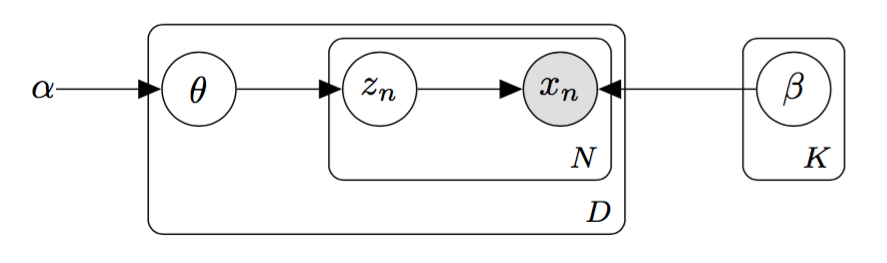
\includegraphics[width=.8\linewidth]{pgm}% standard image
	\captionof{figure}{Bayesian Network Representation of LDA}
	\label{fig:pgm}
\end{minipage}%

\large{
The Bayesian network representation encodes the following generative model:
	\begin{enumerate}
		\item For a set (of discrete observations);
		\begin{enumerate}
			\item Membership proportions vector is drawn ($\theta \sim Dirichlet(\alpha)$)
			\item For each observation (an element of the set)
			\begin{enumerate}
				\item Membership variable is drawn ($z_n \sim Multinomial(\theta)$)
				\item The discrete observation is drawn from ($x_n \sim Multinomial(\beta_{z_n})$)
			\end{enumerate}
		\end{enumerate}
	\end{enumerate}
}


\section{Gibbs Sampling}

\large{
	First note the posterior distribution for $\theta, Z$:
	$$	
	p(\theta, Z | x, \alpha, \beta) = \dfrac{p(\theta, Z, X | \alpha, \beta)}{p(X | \alpha, \beta)}
	$$
	
	where $p(X | \alpha, \beta)$ leads to an intractable integral. 
	
	The key hurdle on the way to a Gibbs sampler is to write the full conditional distributions. In the report, we derive the full conditional distributions in detail, working with a few key ideas:
	
	\begin{itemize}
		\item If we don't require $\theta$ is also learned, we can integrate it out of the joint distribution. We can then use the convenient fact that $p(Z|\alpha, \beta) \propto p(Z, X|\alpha, \beta)$. Then sample from $p(z_n | z_{\neg n}, \alpha, \beta)$ - a collapsed Gibbs sampler.
		
		\item We may also like to infer $\beta$, in which case we would model $\beta$ as drawn from a Dirichlet distribution and sample from it, we do this in Algorithm \ref{alg:coltheta}.
		
		\item It is possible to integrate out $\beta$ as well, in which case one may just draw samples from $Z$, as in Algorithm \ref{alg:collapsed}.
		
		\item We may like to draw samples from all of $\theta, \beta, Z$. We present pseudocode in Algorithm \ref{alg:full}.
	\end{itemize}
}

\section{Algorithms}

\begin{minipage}{\linewidth}
	\captionof{algorithm}{Full Gibbs Sampler}
	\label{alg:full}
	\begin{algorithmic}[1]
			\Function{GibbsLDA}{$X$} \Comment{$X$ is the document-term matrix}
			\State $\beta_k \gets \frac{1}{|V|} $ for all topics $k$
			\State $\theta_m \gets \frac{1}{|K|}$ for all documents $m$
			
			\For{$i = 1$ to NR\_SAMPLES}
				\ForAll{documents $m$}
					\ForAll{words $n$}
						 \State Sample $z'_n | \beta, \theta_m \sim P(z_{n}|\theta_m) P(x_{n}|z_{n}, \beta) $
					\EndFor
					\State Sample $\theta'_m | Z', \beta \sim Dirichlet(\alpha + [N_1, N_2, \dots N_K])$ 
				\EndFor
				\ForAll{topics $k$}
					\State Sample $\beta'_k | Z', \Theta' \sim Dirichlet(\gamma + C_k)$
				\EndFor
			\EndFor
			\EndFunction
	\end{algorithmic}
\end{minipage}

\begin{minipage}{\linewidth}
	\captionof{algorithm}{Gibbs Sampler with Collapsed $\theta$}
	\label{alg:coltheta}
	\begin{algorithmic}[1]
		\Function{GibbsLDACollapsedTheta}{$X$} 
		\State $\beta_k \gets \frac{1}{|V|} $ for all topics $k$
		
		\For{$i = 1$ to NR\_SAMPLES}
		\ForAll{documents $m$}
		\ForAll{words $n$}
		\State Sample $z'_n | \beta \sim \mathcal{M}(\beta_{n} (N_k - 1 + \alpha))$ 
		\EndFor
		\EndFor
		\ForAll{topics $k$}
		\State Sample $\beta'_k | Z'  \sim Dirichlet(\gamma + C_k)$
		\EndFor
		\EndFor
		\EndFunction
	\end{algorithmic}
\end{minipage}

\begin{minipage}{\linewidth}
	\captionof{algorithm}{Fully Collapsed Gibbs Sampler}
	\label{alg:collapsed}
	\begin{algorithmic}[1]
		\Function{GibbsLDACollapsed}{$X$} 
		\For{$i = 1$ to NR\_SAMPLES}
		\ForAll{documents $m$}
		\ForAll{words $n$}
		\State Sample $z'_n | \beta \sim \mathcal{M}(\frac{C_{k,v}  -1 + \gamma_{v}}{\sum_{ v^{\prime} \in \mathcal{X}}C_{k,v^{\prime}} - 1 + \gamma_{v^{\prime}}} (N_k - 1 + \alpha_k))$ 
		\EndFor
		\EndFor
		\EndFor
		\EndFunction
	\end{algorithmic}
\end{minipage}



%----------------------------------------------------------------------------------------
%	OBJECTIVES
%----------------------------------------------------------------------------------------

\section{Conclusion}

We have introduced Bayesian logistic regression. We covered the basic formulation of the method, and moved on to introduce its Bayesian interpretation. We then gave some common priors used in the problem, and discussed MAP estimation. Finally, for approximate inference, we covered Laplace approximation. We concluded that Bayesian logistic regression with priors used purely in a regularization sense does lead to gain in accuracy in text classification, but not to a great extent.

This study left out discussions related to variational methods and Bayesian inference, since they were not directly relevant to the application. They can be the focus of a future study on the subject. For the text classification problem, we can also experiment with more informative priors reflecting prior beliefs on language (such as larger dispersion on longer words). Finally, this study directly tokenizes the text in a bag-of-words manner. The accuracy can be increased significantly with syntactic and morphological parsing of the language.

 %----------------------------------------------------------------------------------------
%	REFERENCES
%----------------------------------------------------------------------------------------

%\nocite{*} % Print all references regardless of whether they were cited in the poster or not
\bibliographystyle{plain} % Plain referencing style
\bibliography{../report/zotero} % Use the example bibliography file sample.bib

%----------------------------------------------------------------------------------------
%	ACKNOWLEDGEMENTS
%----------------------------------------------------------------------------------------

%----------------------------------------------------------------------------------------

\end{multicols}
\end{document}